\section{Understanding Ideal Collaborative Filtering }
\begin{figure*}[t]
  \centering
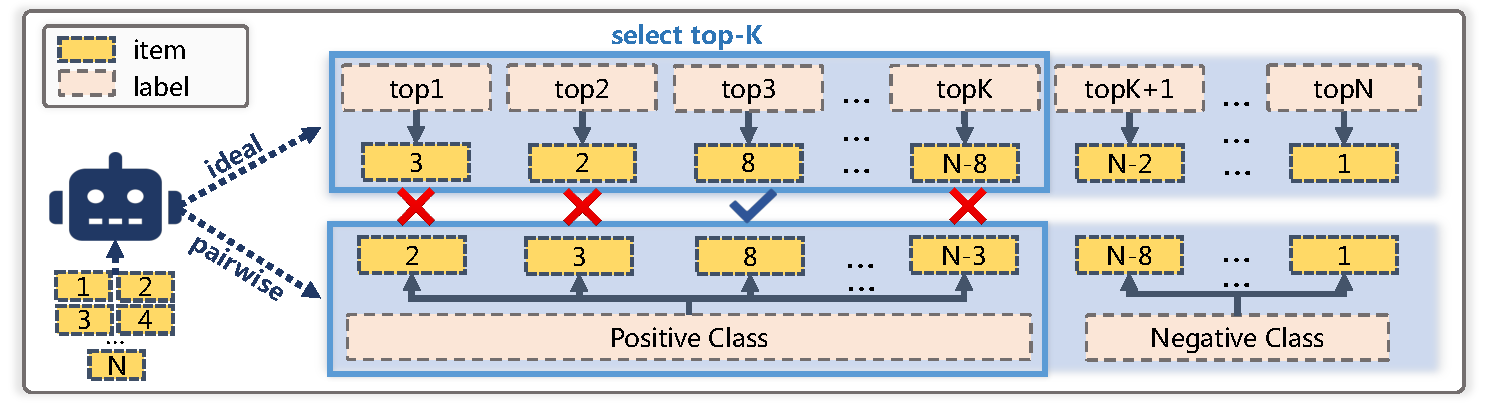
\includegraphics[width=0.8\textwidth]{fig/model.pdf}
  \caption{A comparison between ideal CF and pairwise CF.}
  \label{fig:nips}
  % \vspace{-3mm}
\end{figure*}
According to maximum likelihood estimation, an ideal CF model should be trained by maximizing the posterior probability $\prod_ {u \in U}p(\Theta \mid \Psi_u)$, where $\Psi_u$ represents the full ranking of all items by user $u \in U$. However, in real-world scenarios, this ideal approach is impractical due to the absence of complete ranking information in datasets. Consequently, conventional CF models approximate this by using pairwise loss functions, shifting the optimization objective to maximizing the posterior probability $\prod_ {(u, i_p, i_n) \in D}p(\Theta \mid i_p>_{u} i_n)$. A classic example of this is BPR:
\begin{equation}
\mathcal{L}_{BPR}= -\ln [\sigma(s_u(i_p) - s_u(i_n))],
\label{eq:bpr}
\end{equation}
where $s_u(\cdot)$ denotes the score of an item for user $u$, and $\sigma(\cdot)$ is the $\operatorname{sigmoid}$ function. Models trained with pairwise loss functions are termed pairwise CF models. 

To model the ideal CF, inspired by works such as~\cite{YK20,LWB07}, we propose a novel approach: transforming CF ranking into a multiple ordinal classification problem. Specifically, we hypothesize the existence of $N$ distinct labels $(top1, top2, top3, \ldots, topN)$. For each user $u$, the ideal CF model would assign each item to the appropriate label based on user preference. When making recommendations, these labels are treated as ordinal, with lower $top*$ values indicating higher recommendation priority. Figure~\ref{fig:nips} illustrates this concept. The classification loss in this context can be expressed as:
\begin{equation}
\mathcal{L}_{class} = -\log\frac{\exp(z_t)}{\sum_{v=1}^{N} \exp(z_v)},
\end{equation}
where $z_t$ denotes the score of the target class. Under this framework, pairwise CF can be viewed as a process where each user $u$ considers certain labels (e.g., $top1, top2, \ldots, topK$) as positive samples, while the remaining labels are negative. This comparison highlights that existing pairwise CF methods fall short of achieving ideal CF, exposing a significant gap. This observation raises a critical question: \textbf{Is there a connection between optimizing ideal CF and existing metrics (e.g., NDCG)}? While these metrics are not without flaws, they have proven effective in both practical and theoretical settings. Therefore, it is neither practical nor advisable to disregard them entirely~\cite{PCH24}. Understanding the relationship between ideal CF and traditional metrics is essential.
\begin{theorem}
\label{th:2}
Optimizing ideal CF is a sufficient but not necessary condition for optimizing NDCG.
\end{theorem}

\begin{proof} 
For convenience, we analyze discounted cumulative gain (DCG, with NDCG being its normalized version). DCG is defined as:
\begin{equation}
    DCG_{K} = \sum^{K}_{j=1} \frac{\mathbb{I}(i_{j} \in \mathcal{P})}{\log(j+1)}, 
\end{equation}
where $\mathbb{I}(\cdot)$ is an indicator function, and $\mathcal{P}$ represents the ground truth set of positive items.

\textbf{Sufficient Condition (if part):} If $\Psi_u$ achieves ideal CF, it will rank all positive items at the top, thereby satisfying:
\begin{equation}
\{\Psi_u(1), \Psi_u(2), \ldots, \Psi_u(K)\} = \mathcal{P}.
\end{equation}
This implies that ideal CF $\implies \max DCG_{K}$.

\textbf{Necessary Condition (only if part):}
% Let $\mathcal{P}$ achieve the maximum $DCG_{K}$. 
We can construct a different ranking $\Psi_u^{\prime}$ such that:
\begin{equation}
\forall (j<K), \Psi_u^{\prime}(j) = \Psi_u(j+1), \Psi_u^{\prime}(K)= \Psi_u(1).
\end{equation}
Clearly, ${\Psi_u^{\prime}(1),\Psi_u^{\prime}(2),\Psi_u^{\prime}(3),\ldots \Psi_u^{\prime}(K)} = \mathcal{P}$, satisfying the maximum DCG${K}$. However, $\Psi_u \neq \Psi_u^{\prime}$, meaning that maximizing DCG${K}$ does not necessarily imply ideal CF.
\end{proof}
